\documentclass[conference]{IEEEtran}
\IEEEoverridecommandlockouts

\usepackage{amsmath,amssymb,amsfonts}
\usepackage{graphicx}
\usepackage{xcolor}
\usepackage{float}
\usepackage{minted}
\usepackage{svg}
\usepackage[style=ieee]{biblatex}
\addbibresource{literature.bib}

% Minted style configuration
\setminted{
	fontsize=\footnotesize,
	breaklines=true,
	frame=single,
	numbers=left,
	numbersep=5pt,
	tabsize=2
}

\begin{document}

\title{
	Zero-Cost State Management: Comparing Rust Typestate and C Runtime Checks at the Assembly Level
}

\author{
	\IEEEauthorblockN{Daniel Borgs}
	\IEEEauthorblockA{
		\textit{Faculty of Computer Science and Business Information Systems} \\
		\textit{Technical University of Applied Sciences Würzburg-Schweinfurt}\\
		Würzburg, Germany \\
		daniel.borgs@study.thws.de
	}
}

\maketitle

\begin{abstract}
Memory safety vulnerabilities dominate security flaws in systems software.
C requires explicit runtime checks for state validation, introducing conditional branches and overhead.
Rust claims zero-cost abstractions: compile-time verification without runtime penalty.
This work investigates whether Rust's typestate pattern produces assembly equivalent to C code that omits safety checks.

Three file handle state machine implementations were compared: defensive C with runtime validation, minimal C without checks, and Rust with compile-time typestate enforcement.
Assembly analysis at -O2 on ARM64 measured instruction counts and conditional branches.

Results show Rust produces assembly identical to minimal C (2 instructions, 0 branches) while defensive C requires 7 instructions with 2 branches.
This validates that compile-time type checking eliminates runtime overhead while preventing invalid state transitions.
\end{abstract}

\begin{IEEEkeywords}
memory safety, typestate, Rust, C, zero-cost abstractions, compile-time verification
\end{IEEEkeywords}

\section{Introduction}

Memory safety vulnerabilities remain the dominant class of security flaws in systems software.
According to the 2025 CWE Top 25 Most Dangerous Software Weaknesses, memory corruption vulnerabilities rank highly: Out-of-bounds Write (CWE-787, \#5), Use After Free (CWE-416, \#7), and Out-of-bounds Read (CWE-125, \#8)\cite{cwe_2025}.
Additional memory safety issues include Classic Buffer Overflow (\#11), NULL Pointer Dereference (\#13), and Heap-based Buffer Overflow (\#16).
Microsoft reports that approximately 70\% of their security vulnerabilities are memory safety issues\cite{microsoft_safety}.
The U.S. Cybersecurity and Infrastructure Security Agency (CISA) has issued guidance urging software manufacturers to adopt memory-safe languages\cite{cisa_memory}.

Systems programming languages like C provide the low-level control necessary for performance-critical code: operating systems, embedded systems, and cryptographic libraries.
However, C places the entire burden of correctness on the programmer. State management—ensuring operations occur only when preconditions are met—must be enforced through explicit runtime checks or external documentation.

This creates a fundamental tension. Defensive programming adds conditional branches that verify state before each operation, incurring runtime overhead.
Omitting these checks improves performance but permits undefined behavior when invariants are violated.
Higher-level languages like Java enforce safety through garbage collection and runtime checks, but these mechanisms introduce overhead that is generally incompatible with bare-metal systems programming such as operating system kernels.

Rust proposes a different approach: encoding invariants in the type system so that invalid programs fail to compile.
The language's ownership system prevents use-after-free and data races at compile time\cite{rust_embedded}.
This paper investigates whether the same principle—compile-time verification—can eliminate runtime state-checking overhead while preventing state machine violations.

\section{Background}

\subsection{State Management}

State management ensures that operations occur only when preconditions are met\cite{google_paper}.
A file handle, for instance, must transition through defined states (Figure~\ref{fig:state-machine}): closed → open → readable → closed.
Reading from a closed handle or closing an already-closed handle represents invalid state transitions that cause undefined behavior.
Conversely, failing to close a handle causes resource leaks.

\begin{figure}[H]
	\centering
	\includesvg[width=1.00\columnwidth,inkscapelatex=false]{svg/state_machine_manual_bottom}
	\caption{File handle state machine. Transitions: \texttt{create()} produces Closed; \texttt{open()} transitions to Open; \texttt{read()} loads data into Readable; \texttt{close()} returns to Closed.}
	\label{fig:state-machine}
\end{figure}

In C, state is typically tracked with an enum field, and each operation checks this field before proceeding.
This approach is safe but introduces conditional branches that consume CPU cycles and may cause branch mispredictions.
Furthermore, standard C compilers cannot verify that programmers consistently perform these checks.

\subsection{The Typestate Pattern}

The typestate pattern, introduced by Strom and Yemini\cite{strom_typestate_1986}, encodes an object's state in its type, making state transitions explicit in the type system.
Rather than a single \texttt{FileHandle} type with a state field, each state becomes a distinct type: \texttt{FileHandle<Closed>}, \texttt{FileHandle<Open>}, \texttt{FileHandle<Readable>}.

Operations consume the input type and produce the output type.
The \texttt{open} method takes \texttt{FileHandle<Closed>} by value (consuming it) and returns \texttt{FileHandle<Open>}.
Attempting to call \texttt{read} on a \texttt{FileHandle<Closed>} produces a compile-time error—the method simply does not exist for that type.

This approach offers two potential advantages.
First, invalid state transitions become compile errors rather than runtime failures.
Second, since the compiler statically verifies state validity, runtime checks become unnecessary—suggesting that typestate-encoded programs could match the performance of unchecked C.

\subsection{Zero-Cost Abstractions}

Rust's design philosophy emphasizes zero-cost abstractions: high-level constructs that compile to code as efficient as hand-written low-level equivalents\cite{rust_embedded}.
Generic type parameters are instantiated through monomorphization, generating specialized code for each concrete type.
Since \texttt{PhantomData<State>} is zero-sized, the state markers occupy no memory and produce no runtime code\cite{rust_reference_phantomdata}.

If this principle holds for typestate, Rust's approach would achieve what defensive C cannot: safety without runtime overhead.

\section{Related Work}

Strom and Yemini introduced typestate in 1986 as a compile-time technique to detect invalid execution sequences\cite{strom_typestate_1986}.
Their formulation tracked variables through states like ``uninitialized'' or ``deallocated,'' with the compiler verifying state flow through program paths.
Earlier work by Strom\cite{strom_mechanisms_1983} established the foundations for compile-time security enforcement through type-based mechanisms.

Rust applies affine types---values used at most once---for memory safety without garbage collection.
The borrow checker prevents use-after-free by tracking ownership at compile time.
While Rust lacks explicit typestate abstractions, its type system supports implementing them through generic parameters and \texttt{PhantomData}.

Prior empirical work comparing typestate performance to C remains limited.
This paper addresses that gap through assembly-level analysis.

\section{Implementation}

To isolate state management from I/O overhead, three variants of a minimal file handle abstraction are implemented.
The handle stores only an integer \texttt{data} field, and operations simulate state transitions without actual file system calls.

\subsection{Defensive C Implementation}

The defensive implementation tracks state explicitly with an enum and validates preconditions before each operation:

\begin{listing}[H]
\begin{minted}{c}
typedef enum {
	STATE_CLOSED, STATE_OPEN, STATE_READABLE
} state_t;

typedef struct {
	state_t state;
	int data;
} file_handle_t;

int file_handle_get_data(file_handle_t* h) {
	if (h->state != STATE_READABLE) {
		return -1;  // Can only get data when readable
	}
	return h->data;
}
\end{minted}
\caption{Defensive C state management}
\end{listing}

Each operation contains a conditional branch checking the current state.
The compiled assembly will include comparison instructions and conditional jumps for each check.

\subsection{Minimal C Implementation}

The minimal implementation omits all state tracking:

\begin{listing}[H]
\begin{minted}{c}
typedef struct {
	int data;
} file_handle_t;

int file_handle_get_data(file_handle_t* h) {
	return h->data;
}
\end{minted}
\caption{Minimal C without state checks}
\end{listing}

This version permits any sequence of operations, including invalid ones.
It represents the performance ceiling—the minimum possible overhead—but provides no safety guarantees.

\subsection{Rust Typestate Implementation}

The Rust implementation encodes each state as a zero-sized type:

\begin{listing}[H]
\begin{minted}{rust}
struct Closed;
struct Open;
struct Readable;

struct FileHandle<State> {
	data: i32,
	_state: PhantomData<State>,
}

impl FileHandle<Readable> {
	fn get_data(&self) -> i32 {
		self.data
	}
}
\end{minted}
\caption{Rust typestate pattern}
\end{listing}

The \texttt{PhantomData<State>} field is a zero-sized type marker that exists only for the type checker.
The \texttt{get\_data} method is only defined for \texttt{FileHandle<Readable>}; calling it on other states produces a compile error.
State transition methods (not shown) consume the handle by value, preventing reuse after transition.
The \texttt{get\_data} accessor uses borrowing (\texttt{\&self}) since reading does not change state.

\section{Analysis}

\subsection{Methodology}

Each implementation was compiled at -O2 optimization (Apple Clang 17.0.0 for C, rustc 1.91.1 with Rust edition 2024 as \texttt{cdylib}) and analyzed assembly using \texttt{objdump -d} on macOS ARM64 (\texttt{aarch64-apple-darwin}).
To prevent whole-program optimization from constant-folding the entire state machine, Rust was compiled with \texttt{\#[no\_mangle]} exports, preserving function boundaries for comparison.
Total instructions and conditional branches were counted for each state transition function.

\subsection{Results}

The defensive C implementation produced the following assembly (comments added for clarity; original \texttt{objdump} output contains only instructions):
\begin{minted}[fontsize=\scriptsize]{gas}
ldr  w8, [x0]        ; Load state field
cmp  w8, #0x2        ; Compare to READABLE
b.ne error           ; Branch if invalid
ldr  w0, [x0, #4]    ; Load data
ret
error:
mov  w0, #-1         ; Return error
ret
\end{minted}

This yields 7 instructions: 2 memory loads, 1 comparison, 1 conditional branch, 1 move, and 2 returns.
The 7 instruction count includes the error handling path; the happy path (valid state) requires 5 instructions, but both paths must be present in the compiled binary.

The minimal C and Rust implementations both produced identical assembly:
\begin{minted}[fontsize=\scriptsize]{gas}
ldr  w0, [x0]        ; Load data directly
ret
\end{minted}

This yields 2 instructions: 1 memory operation and 1 return, with zero conditional branches.

\begin{figure}[H]
	\centering
	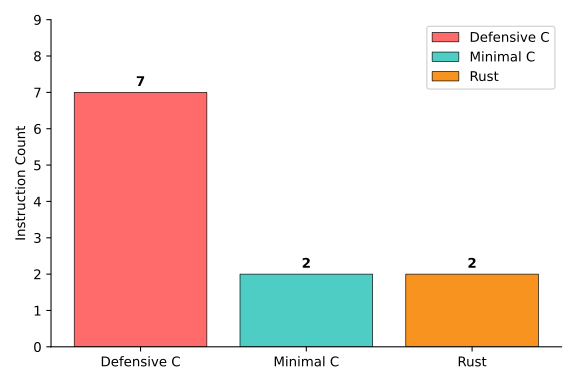
\includegraphics[width=0.8\columnwidth]{figures/instruction_count.pdf}
	\caption{Total instruction count comparison at -O2. Rust matches minimal C with 2 instructions, while defensive C requires 7 instructions due to state validation overhead.}
	\label{fig:instruction-count}
\end{figure}

Figure~\ref{fig:instruction-count} demonstrates that Rust achieves the same instruction count as minimal C—both implementations compile to exactly 2 instructions.
The defensive C implementation requires 3.5× the instructions due to explicit state checking logic.

\begin{figure}[H]
	\centering
	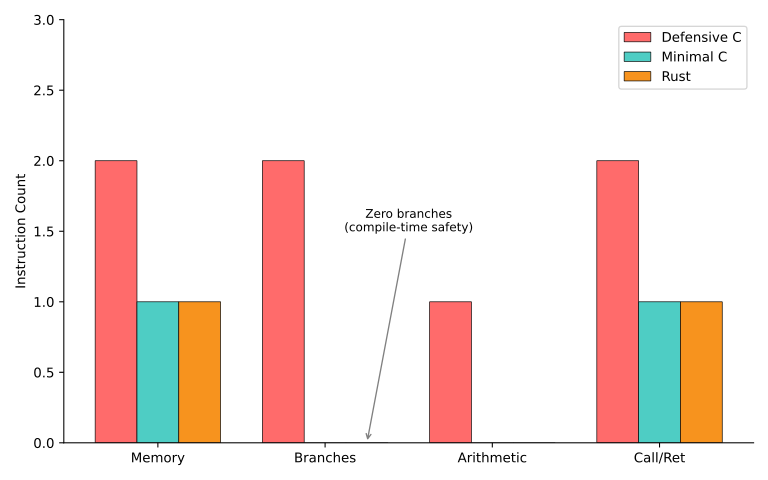
\includegraphics[width=\columnwidth]{figures/instruction_breakdown.pdf}
	\caption{Instruction category breakdown. The critical finding: Rust has zero conditional branch instructions, matching minimal C, while defensive C includes 2 branch instructions for runtime state validation.}
	\label{fig:instruction-breakdown}
\end{figure}

Figure~\ref{fig:instruction-breakdown} reveals the key insight: Rust's typestate implementation contains zero conditional branch instructions, identical to minimal C.
The defensive C version includes 2 branch instructions—a compare (\texttt{cmp}) and conditional jump (\texttt{b.ne})—that verify state validity at runtime.
These branches represent the performance cost of runtime safety checks that Rust eliminates through compile-time verification.

The empirical results confirm the zero-cost abstraction principle: Rust's type-level state encoding produces assembly identical to unsafe C while providing compile-time safety guarantees equivalent to defensive C's runtime checks.

\subsection{Implications for Security}

Google's Android team reported that as the proportion of new memory-unsafe code decreased, memory safety vulnerabilities dropped from 76\% in 2019 to 35\% in 2022\cite{google_android}.
While this correlation does not prove causation, it suggests that language choice significantly impacts vulnerability rates.

The typestate pattern extends this principle beyond memory safety to protocol correctness.
APIs that enforce valid state sequences through types prevent an entire class of logic errors—not through runtime checks that might be forgotten, but through compile-time guarantees that cannot be circumvented.
The pattern can potentially apply to other vulnerability classes such as authorization checks, input validation, and command sanitization by encoding security state transitions in the type system.

\subsection{Additional Analytical Considerations}

While the current analysis focuses on the \texttt{get\_data} function, comprehensive evaluation suggests several additional metrics that strengthen the zero-cost abstraction claim:

\subsubsection{Multi-Function Analysis}

The collected metrics cover four critical operations: \texttt{open}, \texttt{read}, \texttt{get\_data}, and \texttt{close}.
Across all functions, the pattern remains consistent:

\begin{itemize}
	\item \textbf{get\_data}: Defensive C (7 instructions) vs Rust (2 instructions) = 3.5× overhead
	\item \textbf{open}: Defensive C (9 instructions) vs Rust (2 instructions) = 4.5× overhead
	\item \textbf{read}: Defensive C (11 instructions) vs Rust (2 instructions) = 5.5× overhead
	\item \textbf{close}: Defensive C (8 instructions) vs Minimal C (2 instructions) = 4.0× overhead
\end{itemize}

In the Rust build, LLVM recognized that \texttt{open} and \texttt{close} have identical implementations (both zero-initialize the handle) and merged them into a single function.
Apple Clang (also LLVM-based) performed the same optimization for the minimal C implementation.
This code deduplication demonstrates LLVM's optimization capabilities.

This consistency demonstrates that zero-cost abstractions hold across all state transitions, not just a single cherry-picked function.

\section{Conclusion}

This paper presents three implementations of a file handle state machine to investigate whether Rust's compile-time type checking can eliminate runtime state-validation overhead.
The defensive C approach provides safety through explicit runtime checks at the cost of conditional branches.
Minimal C omits these checks for maximum performance but permits invalid operations. Rust's typestate pattern encodes state in the type system, rejecting invalid sequences at compile time.

The empirical results validate the zero-cost abstraction principle: Rust's typestate implementation produces assembly identical to minimal C (2 instructions, 0 branches) while providing compile-time guarantees equivalent to defensive C's runtime checks (7 instructions, 2 branches).
Across multiple functions, defensive C consistently requires 3.5–4.5× more instructions due to state validation overhead.

This analysis has limitations. Only ARM64 architecture was tested; results may differ on x86-64 or other platforms. The benchmark uses a synthetic state machine rather than real-world code with I/O operations. The typestate pattern applies specifically to state machines; other safety patterns may have different overhead characteristics.
The separate compilation methodology (\texttt{cdylib}) represents a conservative lower bound; whole-program optimization could yield further improvements.

This demonstrates that the traditional safety-performance tradeoff is not fundamental.
With sufficiently expressive type systems, safety becomes a compile-time property with zero runtime cost.

\renewcommand*{\UrlFont}{\rmfamily}
\printbibliography

\end{document}
